Visual Solutions is a Norwegian company in the BB Visual Group\footnote{http://www.bbvisualgroup.com/}. Their primary business is within the integration of operations for the oil and gas industry, with customers located all over the world. They create solutions enabling collaboration across organisation units and geographic locations.

\subsection{Virtual Arena}
One of Visual Solutions applications is Virtual Arena\cite{solutions_b2_virtual_2014}, which from now on will be referred to as \gls{va}. VA is a powerful and interactive tool that allows for high-performance application sharing, with audio and video communication from a 3D shared scene as seen in Figure \ref{fig:vsva-3d-scene}.
\\
\begin{figure}[here]
\centerline{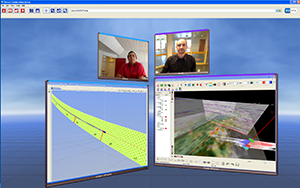
\includegraphics[scale=0.6]{virtualarena.png}}
\caption{Virtual Arena 3D shared scene}
\label{fig:vsva-3d-scene}
\end{figure}

% VA supports many-to-many collaborative scenarios by utilizing a media server.

VA is an application that Visual Solutions has created for doing visual collaboration over IP. The architecture of VA is visualized in Figure \ref{fig:vsva-architecture}. The application uses a media server that serves multiple purposes. It acts as a \gls{mcu}, applies mitigation strategies for scenarios with limited bandwidth, and also sharing of applicaton data. Mitigation strategies can f.ex be reducing the video bitrate to adjust and adapt for poor connections. By utilizing a media server VA can support for a lot of incoming and outgoing streams. A client can subscribe to multiple streams of audio/video and applications. There is a lot of advanced behaviour in this system, but I will not go into specific details, I will only provide a general overview. In the next subsections the different parts of the architecture in Figure \ref{fig:vsva-architecture} will be described with the necessary information required to understand the practical problem this thesis will try to solve. 

\begin{figure}[here]
\centerline{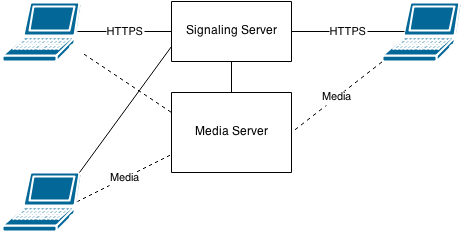
\includegraphics[scale=0.6]{virtualArena-architecture.png}}
\caption{Virtual Arena systems architecture}
\label{fig:vsva-architecture}
\end{figure}

\subsubsection{Signaling}
VA has a proprietary way of doing signaling and the server authenticates users \gls{guid}'s via Kerberos\footnote{Kerberos is a computer network authentication protocol} over HTTPS. This is where the clients send messages to the media server describing which streams they want to subscribe to. Streams are recognized by the their \gls{ssrc}, which is defined in the header packets of the media streams. All the SSRCs are registered in the signaling server. Communication between peers and the media server is done by opening up ports in the firewall to listen for incoming TCP and UDP connections. These ports are preconfigured manually for this application. The media server can receive incoming streams, mix them, and route the media to all peers connected.

\subsubsection{Transport}
VA uses raw \gls{rtp} streams over UDP together with a \gls{rtcp} connection. This is basically the standard protocols used for transmitting real-time media in any communication system. RTCP is used for providing statistics and control information for the RTP flow. There will be more details about the RTP protocol in the upcoming sections.

\subsubsection{Media}
VA uses patent-free codecs for audio and video. It uses Speex\footnote{The Speex Codec Manual - http://www.speex.org/docs/manual/speex-manual.pdf} for audio, and Theora\footnote{Theora Specification - http://theora.org/doc/Theora.pdf} for video. The Speex codec is designed for high quality speech and low bitrate, which is perfect for audio communications. It supports both narrowband and wideband sampling rates in the same bit-stream\cite{speex}, which allows for minimizing bandwidth and an adaptable sound quality. The Theora codec is a common choice in enterprise systems, it is less CPU-intensive than the popular H.264 codec\cite{theora}, which is licensed by Cisco. Theora is also license free, however H.264 offers the added benefits of hardware acceleration in a lot of graphic cards, and Cisco has recently announced that they will make H.264 open-source\cite{h264-free}, which will effectively make the codec free to use in technologies like \gls{wrtc}.

\subsection{Security}
VA only uses raw RTP streams, because no security is needed. It operates in a closed business environment, so transport level encryption is not necessary, because unidentified peers are not allowed inside the network anyways. The enterprise firewall has very strict polices, only allowing certain kinds of traffic on specific ports.

\subsection*{Summary}
VA operates very much like a typical enterprise comunication system. It uses common transport protocols and codecs, however it's architecture is still very different from the protocols and codecs defined in \gls{rtcweb}, which we will see in the next section.